\documentclass[12pt]{article}
\usepackage[utf8]{inputenc}
\usepackage{graphicx}

\title{Master's thesis proposal}
\author{Cristian Manuel Abrante Dorta}
\date{July 2021}

\begin{document}

\maketitle

\section{Introduction}

Cloud computing is a novel field whose usage had increased dramatically during recent years. For many businesses, including multinational companies and young startups, the possibility of externalizing IT resources to cloud providers, represents an important reduction in their operational costs. This cost reduction represents a major competitive advantage to them because they can use the resources they have available (which in case of startups might be limited) to implement the software or operations that really are part of their value proposition and reducing the infrastructure maintenance costs.\\

One of the big players in the cloud computing sector is Google Cloud. The cloud infrastructure provided by Google offers services that can improve the development process; such as storage space and basic server capabilities, and also elements for advanced deployment and orchestration of web applications and services, such as Google App Engine, which is perfect for deploying \textbf{applications based on microservices}.\\

The microservices pattern had gained popularity during the recent years as it speeds-up the development time by dividing the responsibilities of the different \texttt{services} involved in a system, and therefore reducing the time-to-market. Also, microservices pattern allows to correctly match organizational needs, as the team division can be established depending on the services that they own.\\

There are many multinational companies that uses microservices pattern for the development of their backend services, some examples are Uber, Netflix or Unity. Considering that, most of them had adopted the necessity of creating a single entry point for all their services: an API gateway. Technically speaking, the API Gateway is just another service, whose main functionality is forwarding the queries that are sent from the external user to the corresponding microservice that can return the desired response. Apart from this, the gateway can implement some high-level responsibilities, such as rate limiting, load balancing or header enrichment.\\

\section{Engineering questions}

Monitoring the activity of the gateway is not an easy task, especially in big companies where the number of queries that it receive can be in the order of thousands per minute. Also the monitoring is something that is not only relevant for the gateway development team, but it is something that it is interesting for all the teams whose develop services under its umbrella.\\

Taking into consideration that the premise of this thesis is working with microservices architecture applications deployed in a Google Cloud environment that had adopted an API Gateway as an entry point, the main objective is to determine which would be the optimal way of monitoring the activity of the gateway, taking into account that it receives a very intense traffic and that the results of the monitoring had to be communicated in a visual way using a cross-organization tool. In that sense, creating an effective monitoring system for the application gateway is something that can bring a lot of value for companies that have a microservices application working in high scale.\\

\section{Expected outcomes}

The expected outcome of this project is the creation of an application that can monitor the errors that occurs in the \textbf{Unity Services Gateway}. This gateway is the entry point of all the public and private services that are used on the advertisers side in the Unity Ads Network.\\

\begin{figure}
    \centering
    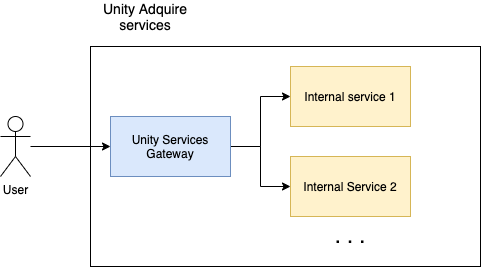
\includegraphics[scale=0.4]{src/proposal/img/diagram-1.png}
    \caption{Current setup of the unity services gateway}
    \label{fig:my_label}
\end{figure}

For the creation of the monitoring application those technologies are going to be used:

\begin{itemize}
    \item \textbf{BigQuery}: Due to the high volume of queries that the gateway handles and the possible amount of errors that can occur in those, it makes sense to use an storage platform that can be scaled to high volumes of data and that can be accessed easily.
    \item \textbf{NodeJS}: The service is written in Javascript and it is using Node.js, so this language and this technology is going to be used for doing the correspondent modifications to it.
    \item \textbf{Grafana}: Grafana is a tool for data visualization and monitoring, it is the standard used in the company so it is going to be used for creating meaningful visualizations for the error events.
\end{itemize}

Taking into consideration the technologies that are going to be used we can create a predefined plan and define the expected outcomes of the project:

\begin{itemize}
    \item Define the structure of the events that are going to be stored in the database. For the proof of concept, the rate limiting error can be used, but this can also be extended to other types of errors in the future.
    \item Add the necessary tables that will contain the events to BigQuery.
    \item Add the functionality of logging the results into BigQuery to the gateway.
    \item Connect Grafana to BigQuery in order to enable error visualization.
\end{itemize}

It is important to remark that this can be considered an iterative process, because as  are developing a software tool, maybe new needs come from different teams or there are some concerns about things that can be improved, so it is important to say that the final result is going to be the result of iterating over the solution.

\end{document}
